\section{Mechanical Design}
\label{sec:background}

\subsection{Structure Design Overview}

\subsubsection{First version}
\par

MAVEN-01 was first designed as a two-tracked, tank-type vehicle platform using two 6V TT gear motors for each track. 
The size of the rover frame platform is 16.8 × 11 cm. The reason why the first body was small is due to the space limitation 
of the printing plate area of the Bambu Lab A1 Mini, which is our 3D printer. During the process, there were two material options: PLA and PETG. 
PETG is cheaper than PLA and offers higher durability and better heat resistance, but it is harder to print and requires careful storage 
due to its humidity-sensitive properties.

\vspace{1.5 em}
\par
We chose PLA for its easier printing process and better print consistency, which is more suitable for rapid prototyping and iterative design. 
PETG might be chosen for more specific missions that require higher durability in harsher environments.

\begin{figure}[H]
    \centering
    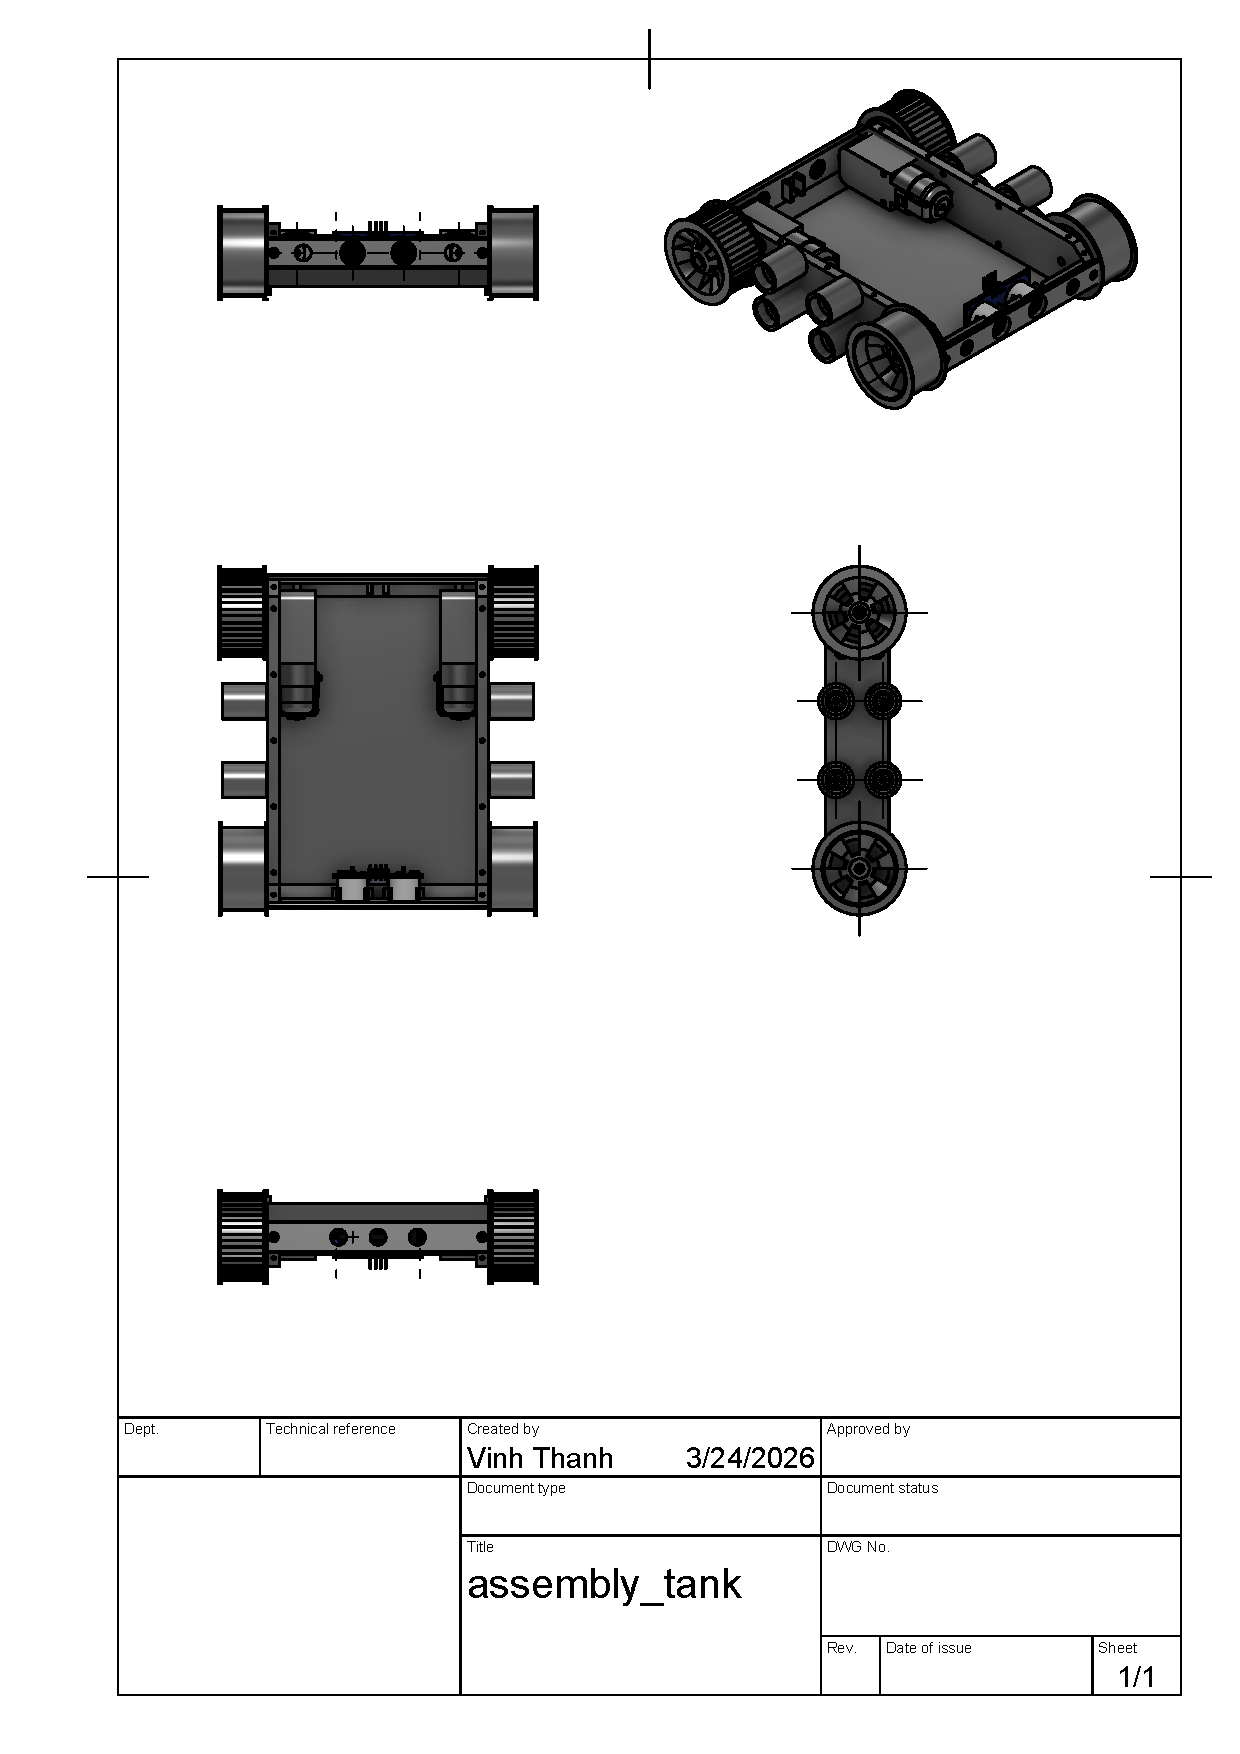
\includegraphics[width=0.75\linewidth]{images/blueprint/maven_01_first_prototype.pdf}
    \caption{Blueprint of MAVEN-01 first prototype}
    \label{fig:first_vers_blueprint}
\end{figure}


\text{Disadvantages}
However, there are some disadvantages in the first design that should be carefully considered. 
Due to the low ground clearance, this design cannot operate effectively in rugged terrain.

Another disadvantage is that the track can slip off the wheels due to the unstable drive wheel. 
In the first design, M4×30 screws and nuts are used to mount the drive wheel and front wheel. 
This design has a weakness: during testing, the screws wore into the wheel holes on the body, 
which caused the drive wheels to loosen over time, making the track structure weaker.

\vspace{1em}
The last weakness of this design is two engines are mounted inside the rover body, which 
occupy a large space, we can put more components inside base body. During operation time, two DC motor 
can generate heat which can effect on micro-control board, also not ideal for PLA body due to not limited heat resistance.


\begin{table}[h]
\centering
\begin{tabular}{|l|c|c|}
\hline
\textbf{Feature} & \textbf{PLA} & \textbf{PETG} \\
\hline
Printability & Very easy & Moderate \\
\hline
Strength & Strong but brittle & Strong and flexible \\
\hline
Temp. Resistance & Low ($\sim$70$^\circ$C) & Moderate ($\sim$85$^\circ$C) \\
\hline
Durability & Low outdoor durability & High UV resistance \\
\hline
Post-Processing & Easy to sand/paint & Harder to sand \\
\hline
\end{tabular}
\caption{Comparison of PLA and PETG specifications}
\label{tab:pla_vs_petg}
\end{table}

\subsubsection{Second Version}

\begin{figure}[H]
    \centering
    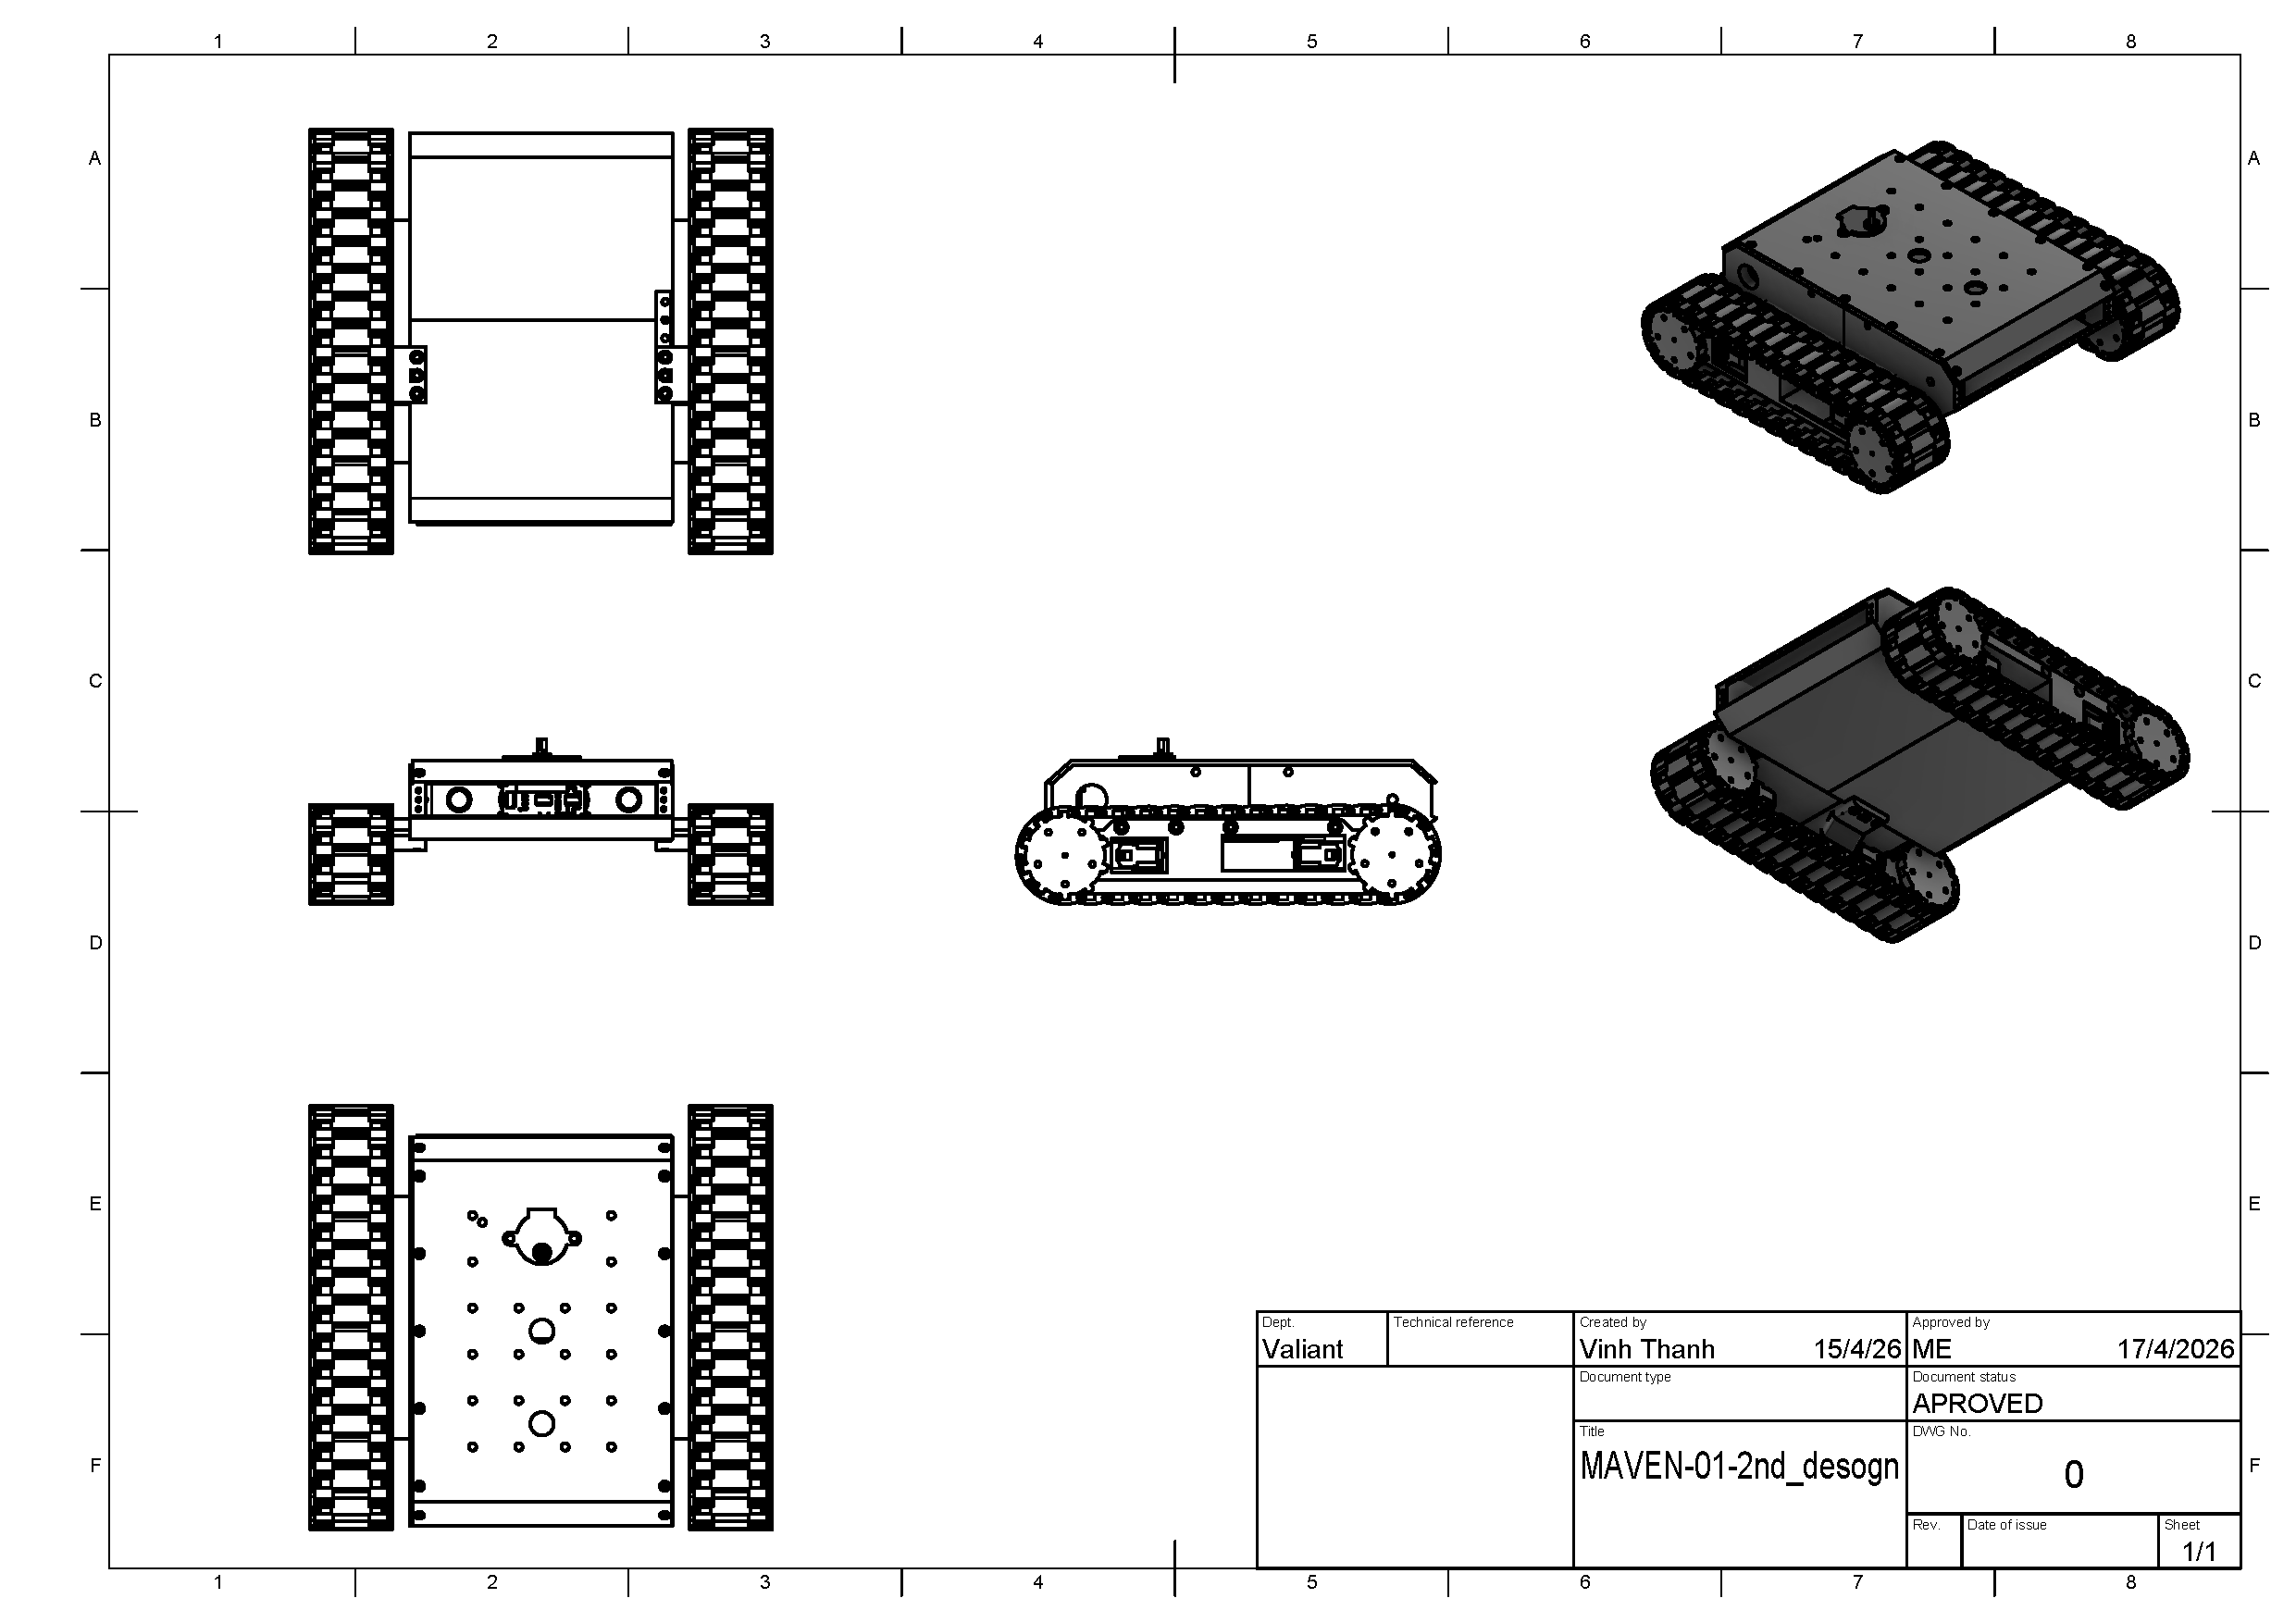
\includegraphics[width=0.95\linewidth]{images/blueprint/Maven-01-2nd-design.pdf}
    \caption{MAVEN-01 second prototype design using separate chassis with chained tracks (Single motor chassis) }
    \label{fig:chasis_1_engine_blueprint}
\end{figure}

\par
In this version, we improve the design  completely to fix the disadvantages of the first design. We move the track system into a separate module,
which allows more space in the base rover body. With the separate track module, the ground clearance can be higher, allowing MAVEN-01 to adapt to different terrain types and rough surfaces.
The \href{https://www.st.com/resource/en/datasheet/l298.pdf}{L298N} motor driver module and gear motor heating problems are also solved by the open-surface chassis design, which allows open-air ventilation to work as a cooling system.
My design inspired by \cite{TankTrack2024} but with some modified for better upgrade in the future.


\subsubsection{Chassis design}
\begin{figure}[H]
    \centering
    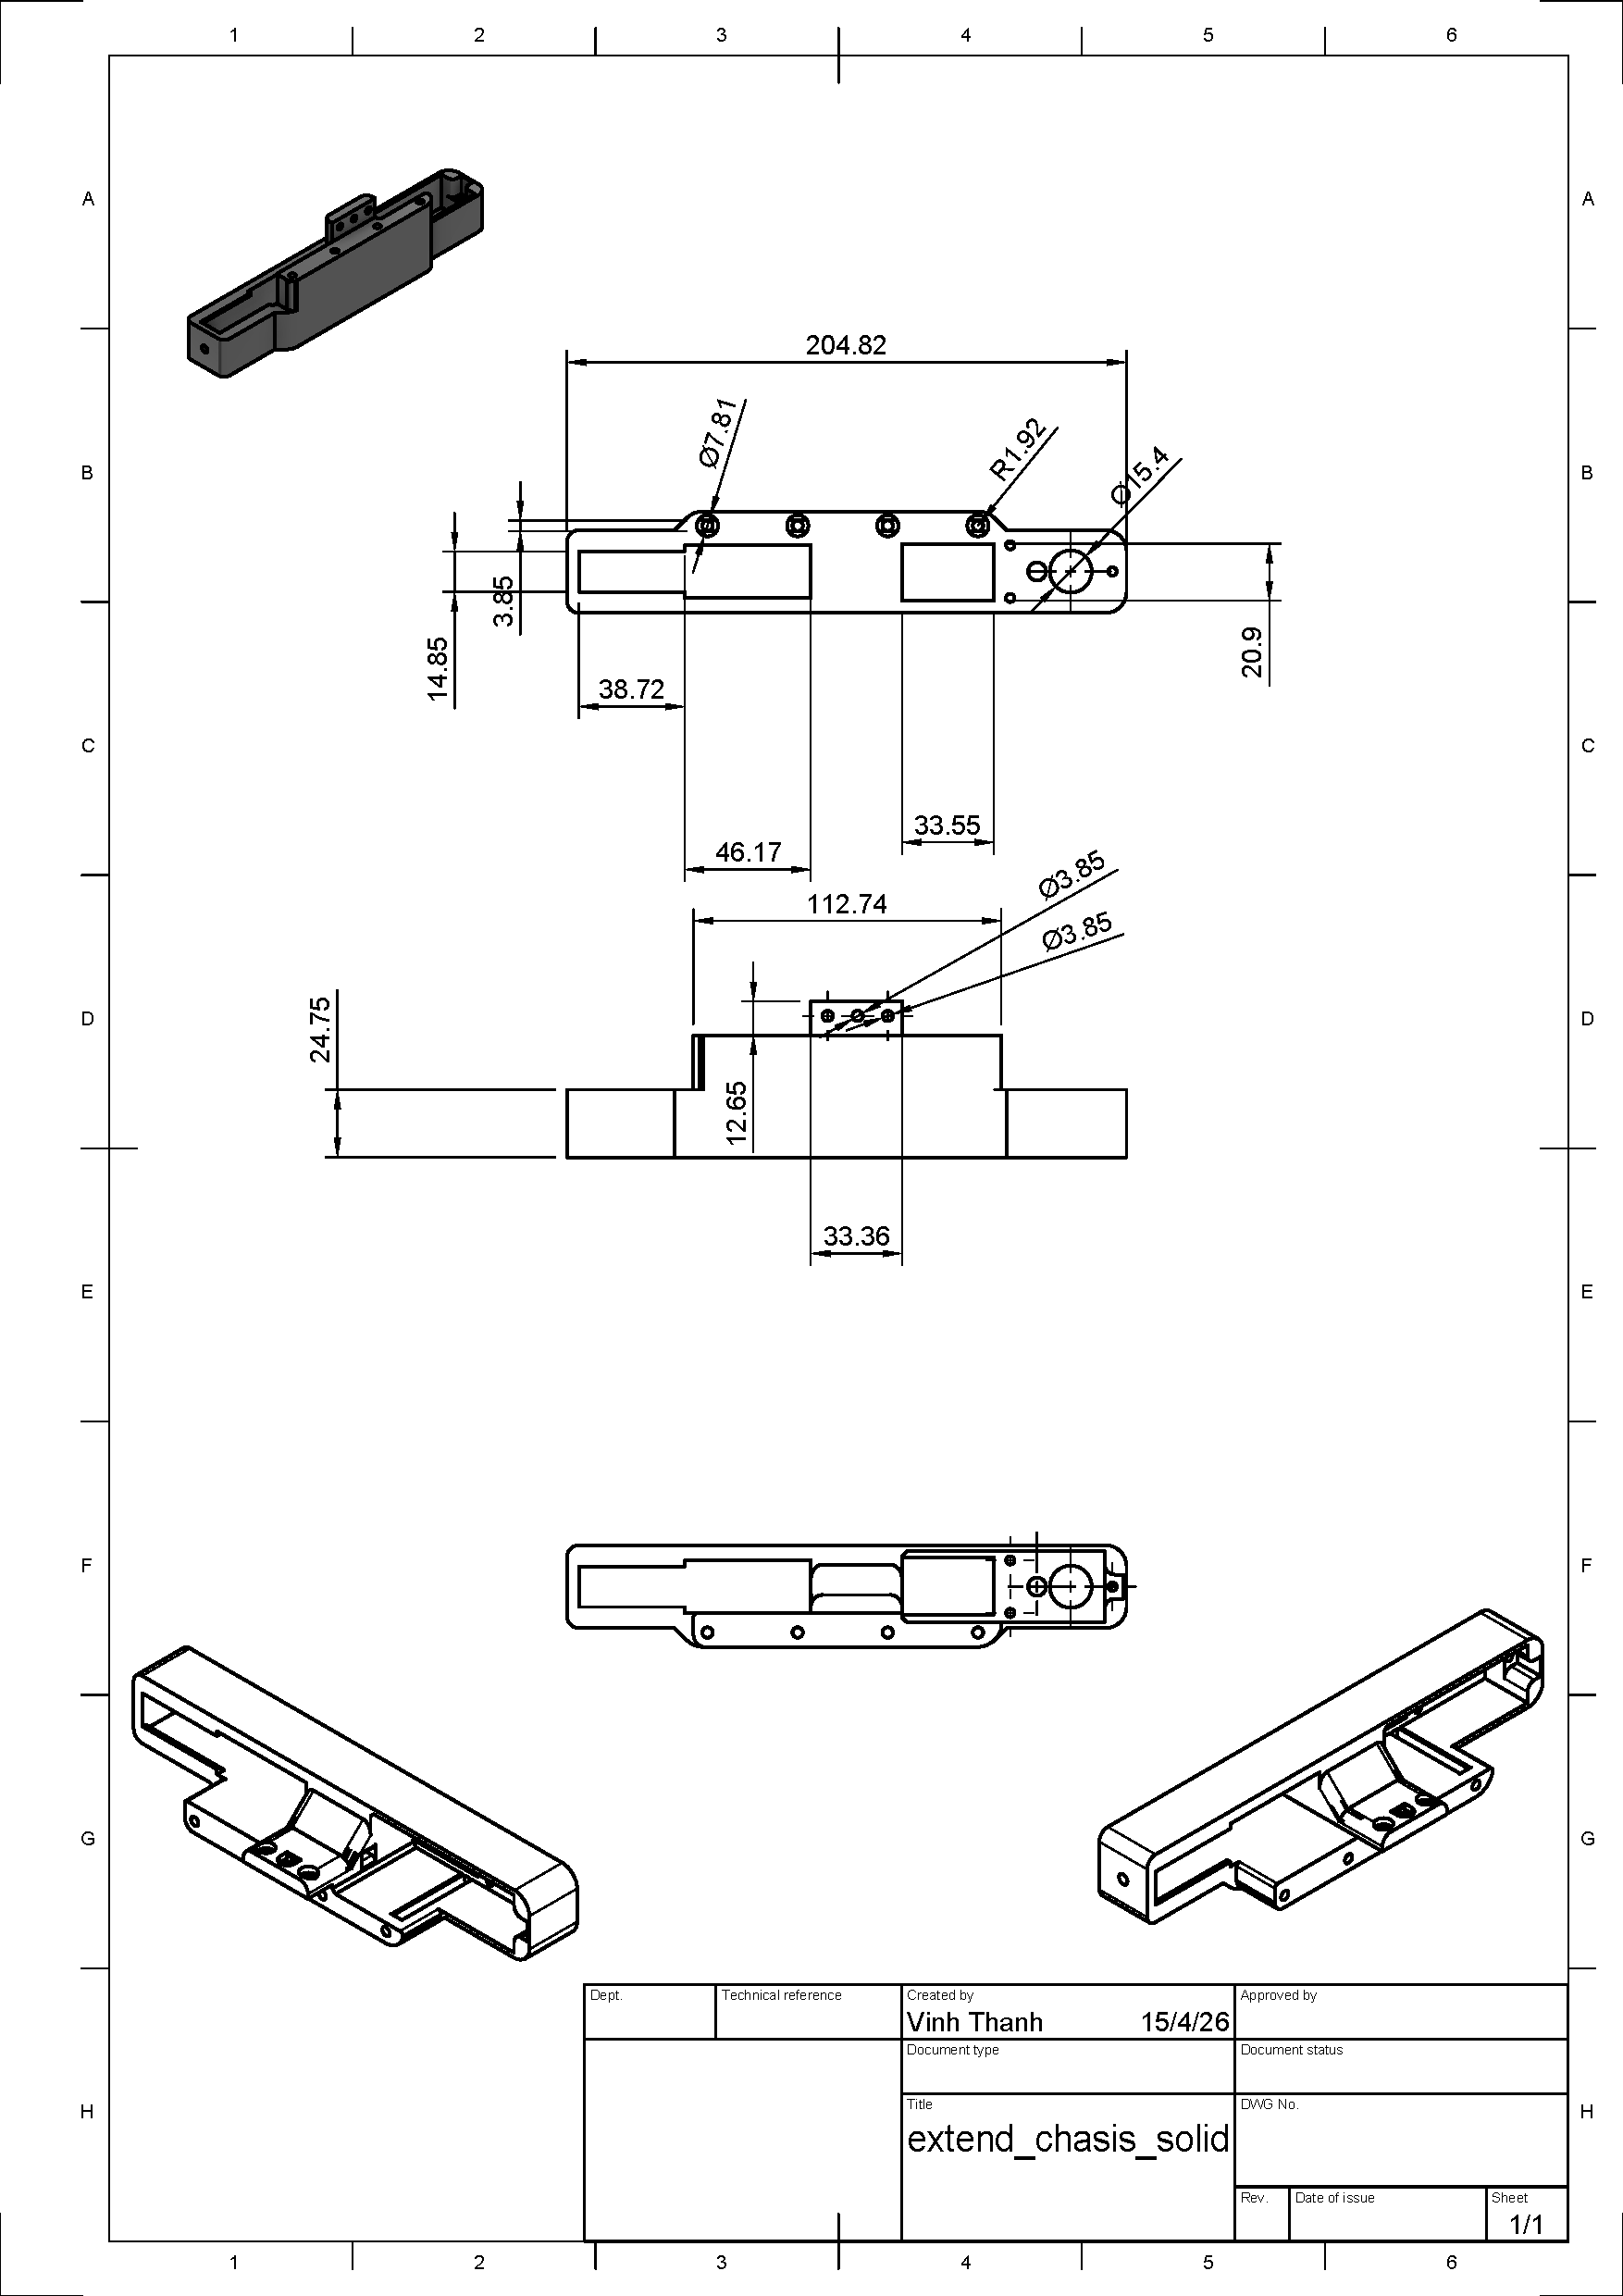
\includegraphics[width=0.9\linewidth]{images/blueprint/chassis_1_engine.pdf}
    \caption{Single motor chassis blueprint for 6V TT gear motor with open surface for motor air cooling }
    \label{fig:chasis_1_engine_blueprint}
\end{figure}

\vspace{2em}
\subsubsection{Drive wheel design}

\begin{figure}[H]
    \centering
    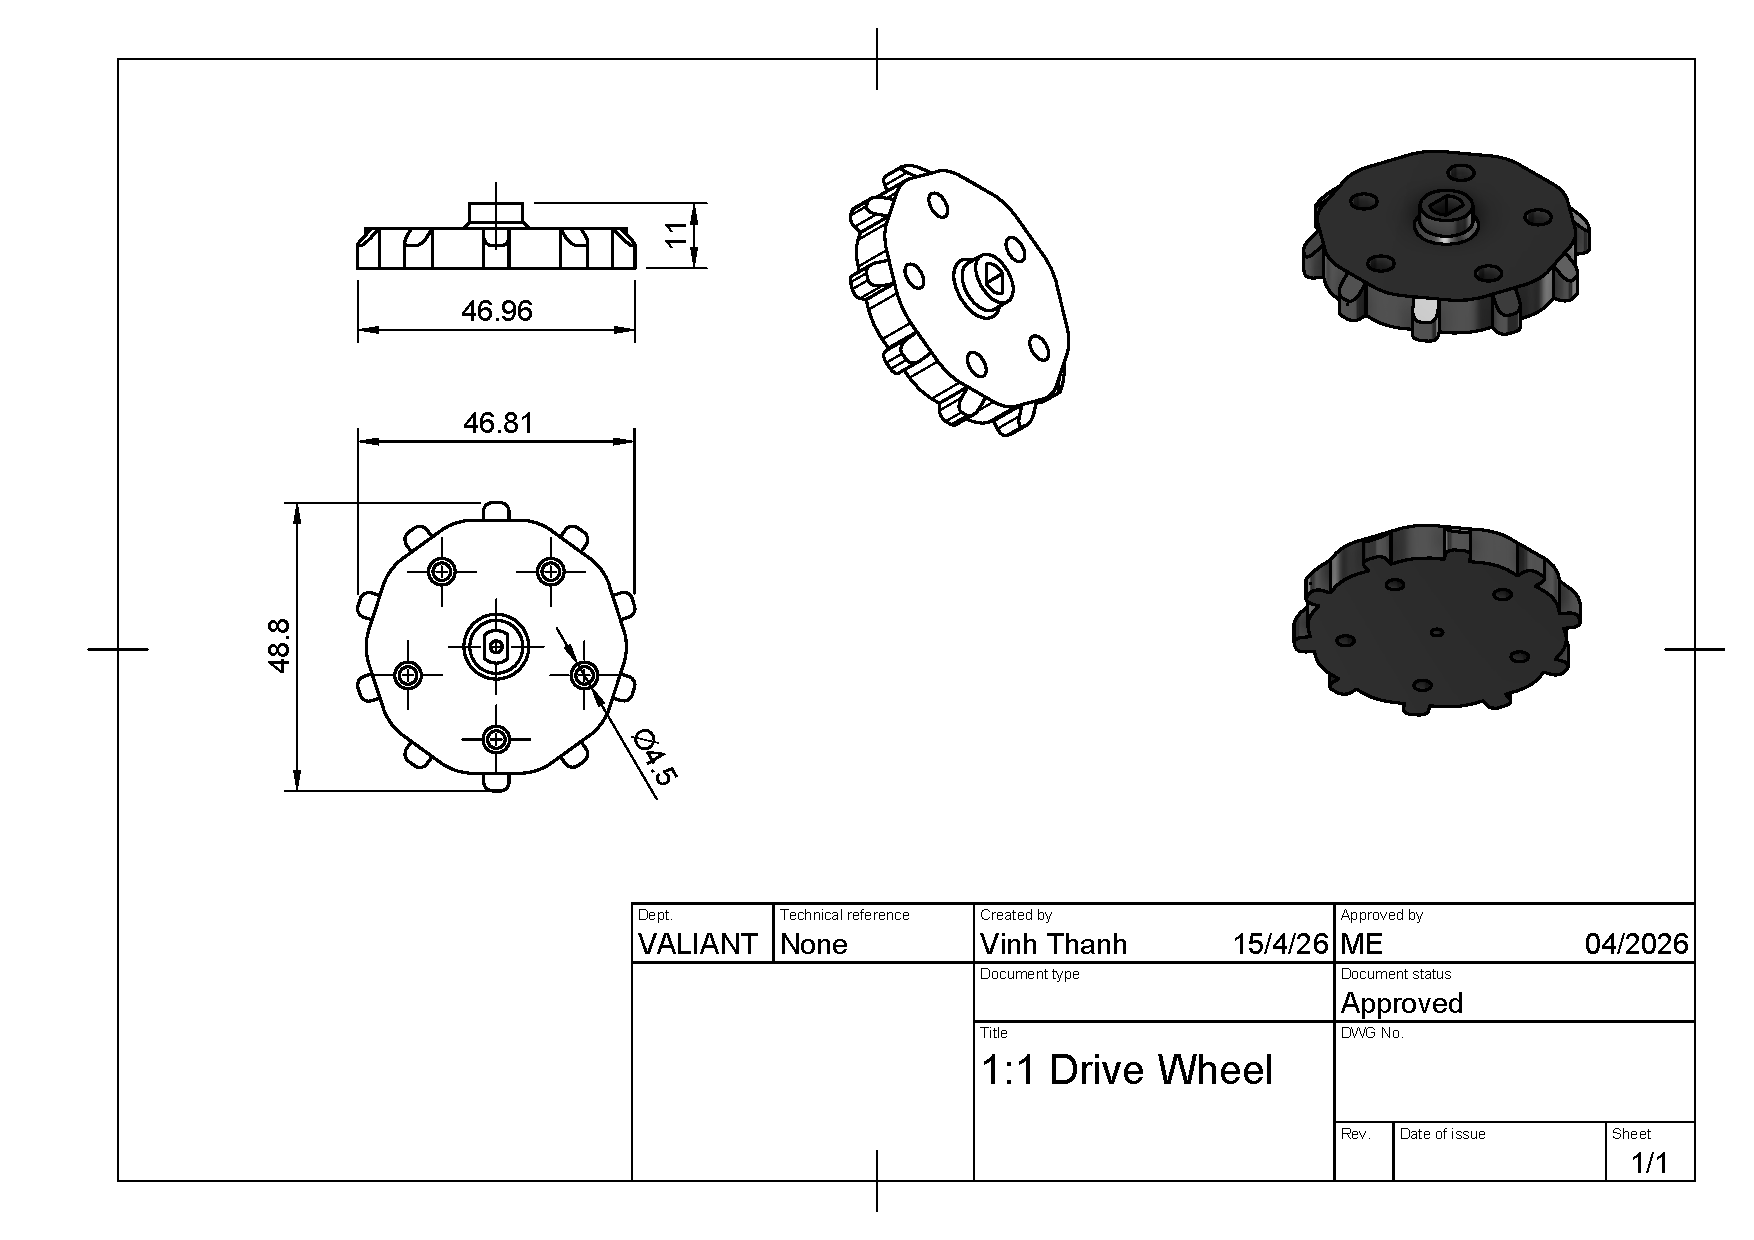
\includegraphics[width=0.8\linewidth]{images/blueprint/drive_wheels.pdf}
    \caption{Driver wheels blueprint for MAVEN-01}
    \label{fig:drive_wheels_blueprint}
\end{figure}

Each TT motor will have two drive wheels act as anchors for track chains attached. Drive wheels can be 
attached info motor axises using glue or M2x10 to M2x12 tap screws. 

\vspace{1em}

\subsubsection{Passive wheel design}
\par
Passive wheel were design to attach 6700zz bearing for smooth rotation, 6700zz has size of 
15x10x4MM, mounted and screwed with M5x10 tap screw and M5 nuts as holding reinforcement. 
\par
\begin{figure}[H]
    \centering
    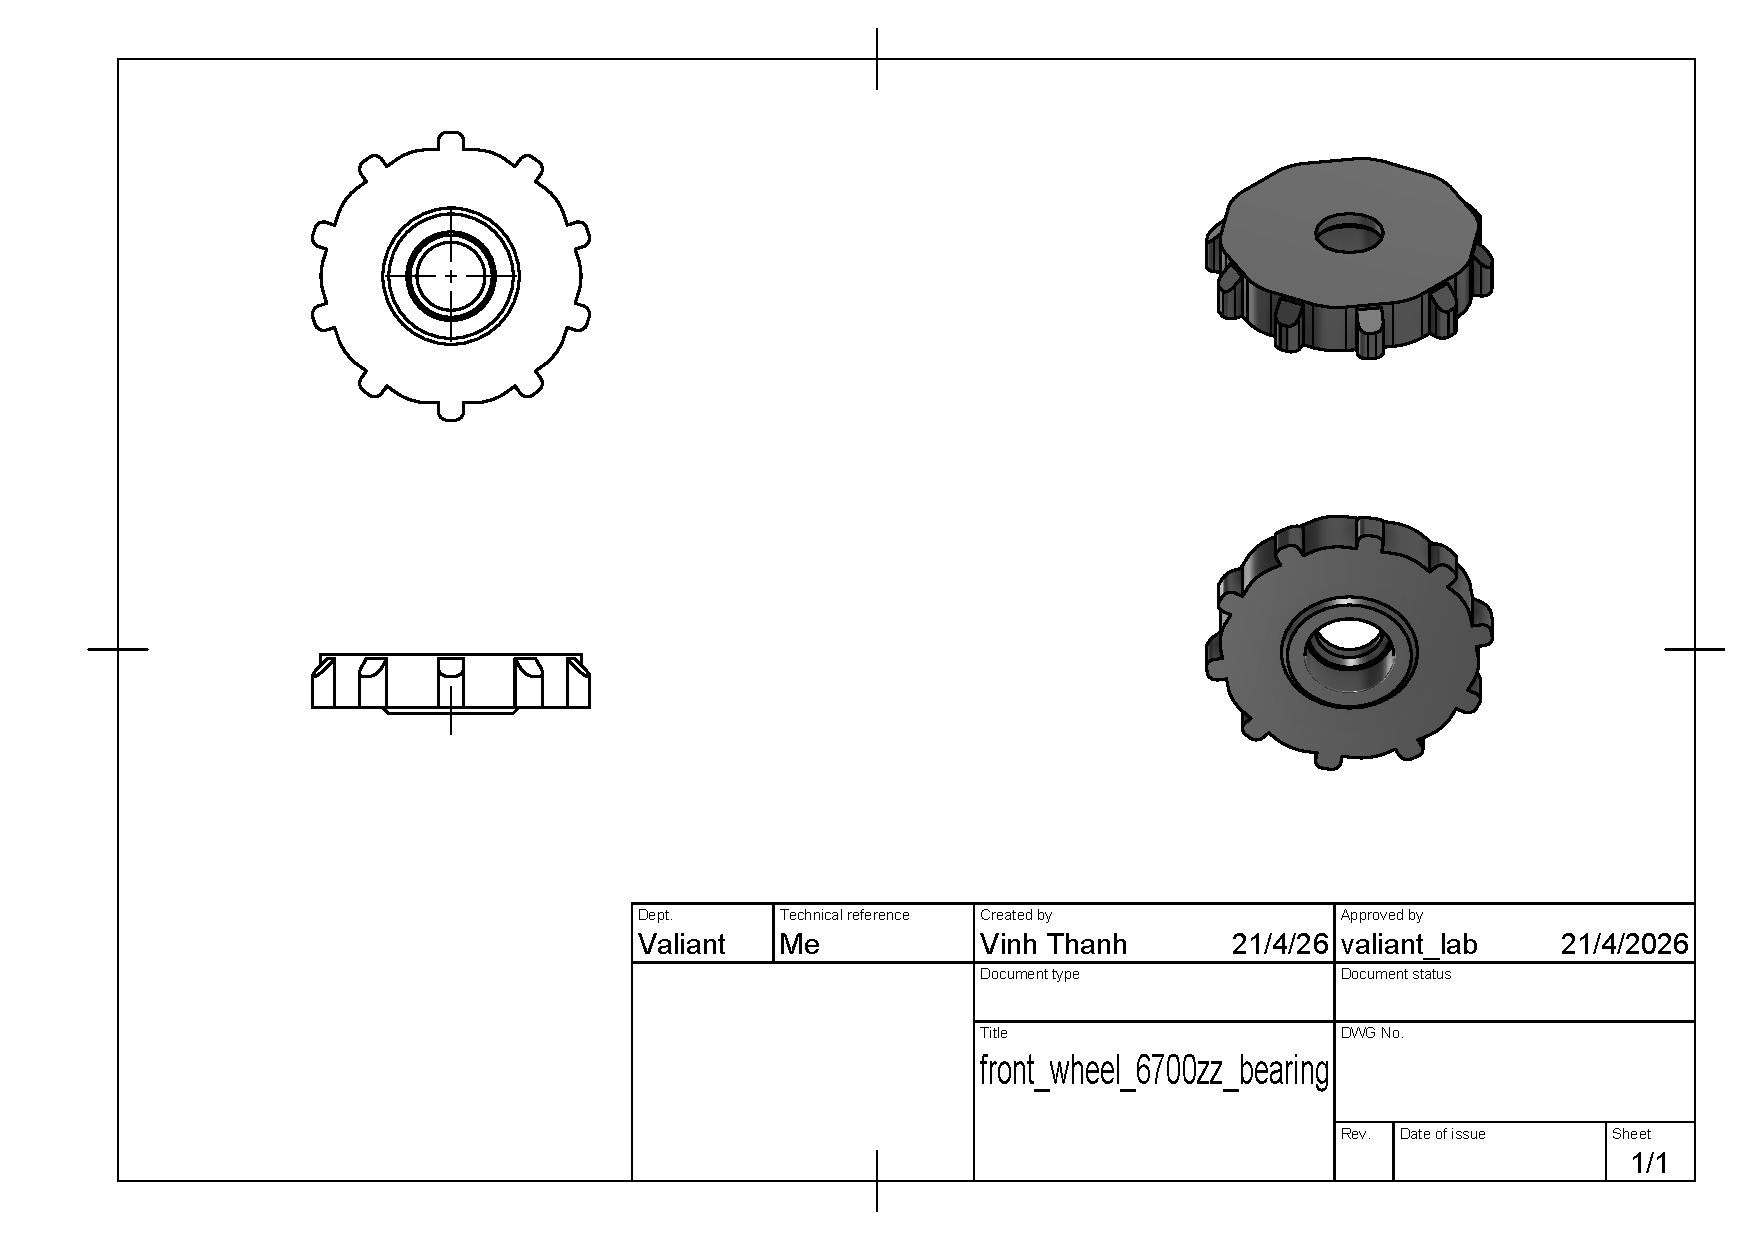
\includegraphics[width=0.80\linewidth]{images/blueprint/front_wheel_6700zz_bearing_oriented.pdf}
    \caption{Front wheels with 6700zz bearingblueprint for MAVEN-01}
    \label{fig:frontwheel_6700zz}
\end{figure}\vspace{1em}


\subsubsection{Front axis}
\vspace{1.5em}

\begin{figure}[H]
    \centering
    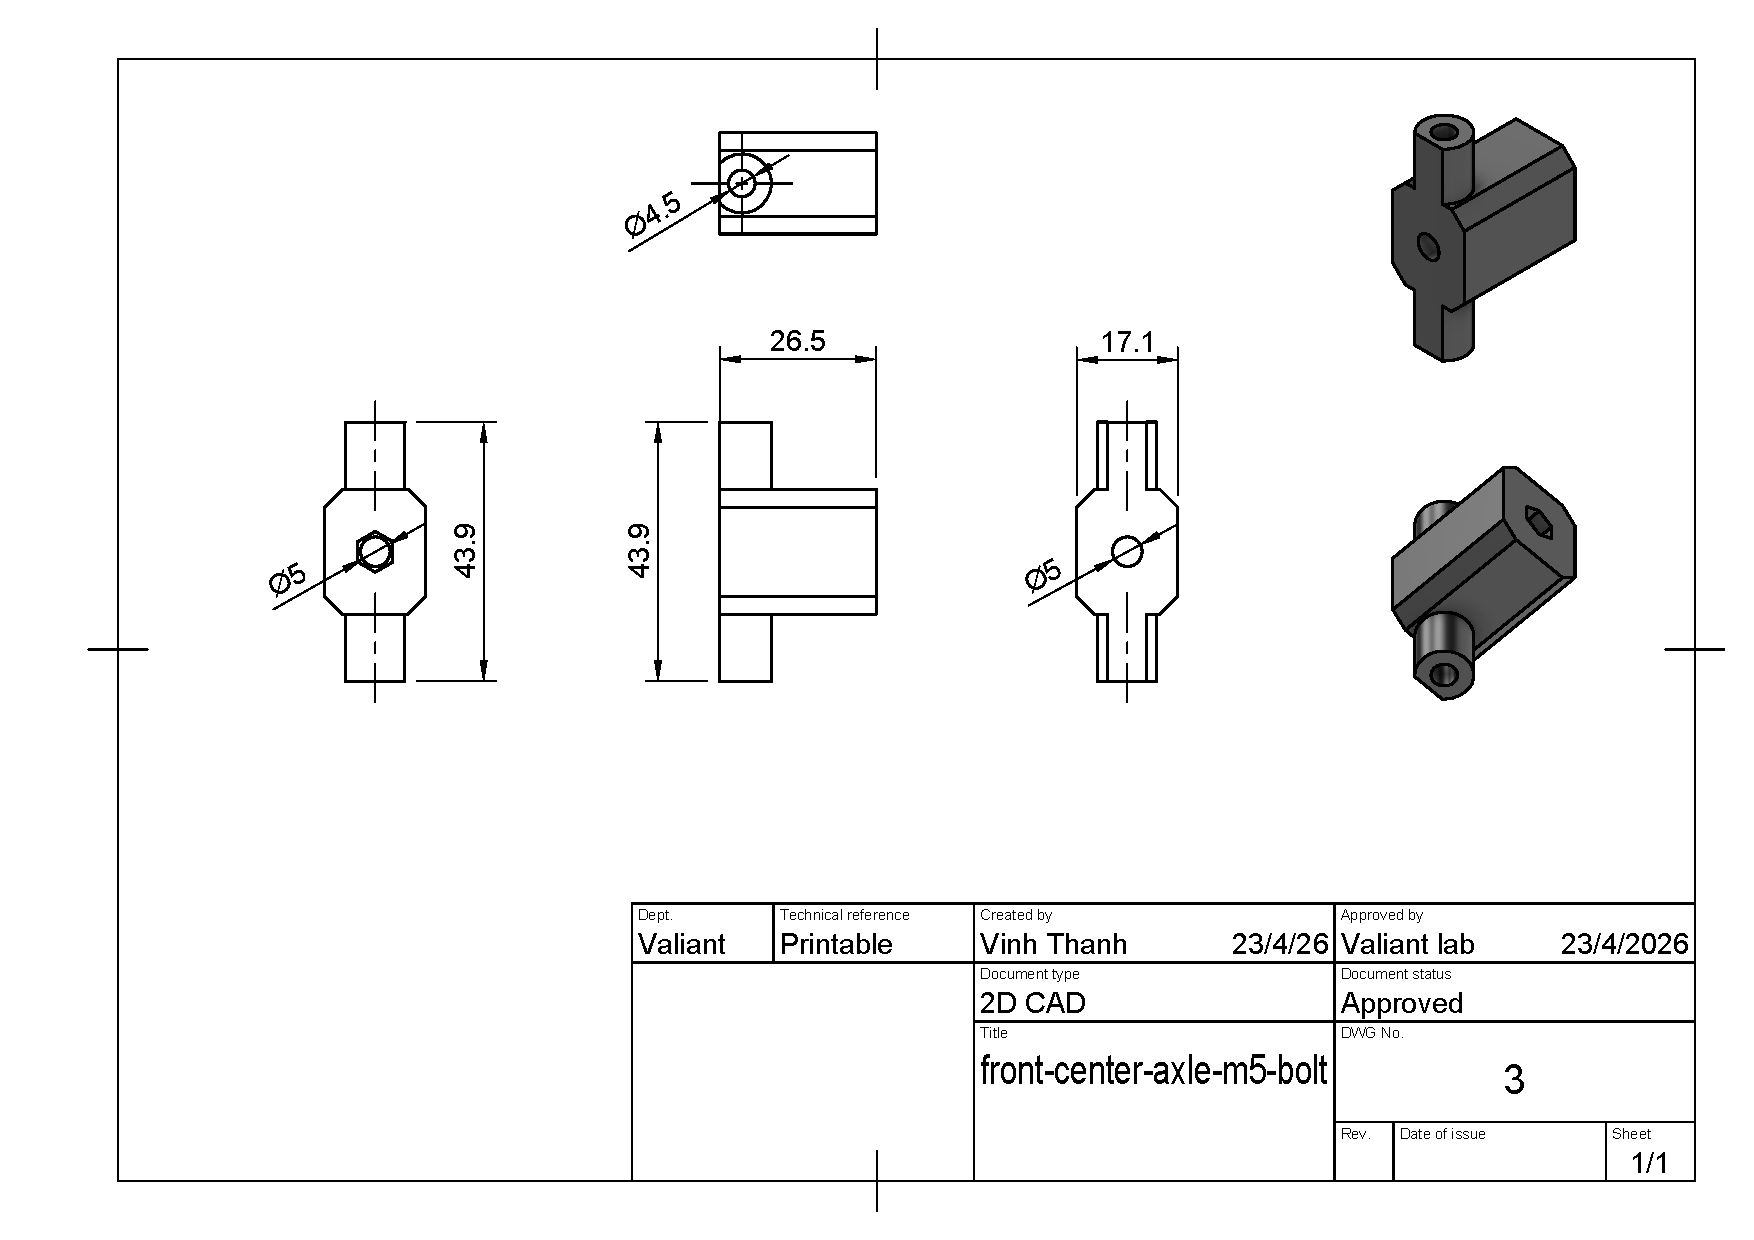
\includegraphics[width=0.78\linewidth]{images/blueprint/front-center-axle-m5-bolt_drawing.pdf}
    \caption{Front axis for front wheels for M5 bolts}
    \label{fig:frontwheel_axis_m5_bolt}
\end{figure}\vspace{1em}

\par
Front wheels of Maven-01 are designed not to be attached directly to the chassis;
they will be attached to a front wheel axis. The reason for separating this part from the chassis is that the front wheels are passive, 
which over time can be abraded. With the front wheels attached to the front axis instead of the chassis, 
they can be easily changed when worn out,and chassis replacement will not be required.


\subsubsection{Track chain}
\begin{figure}[H]
    \centering
    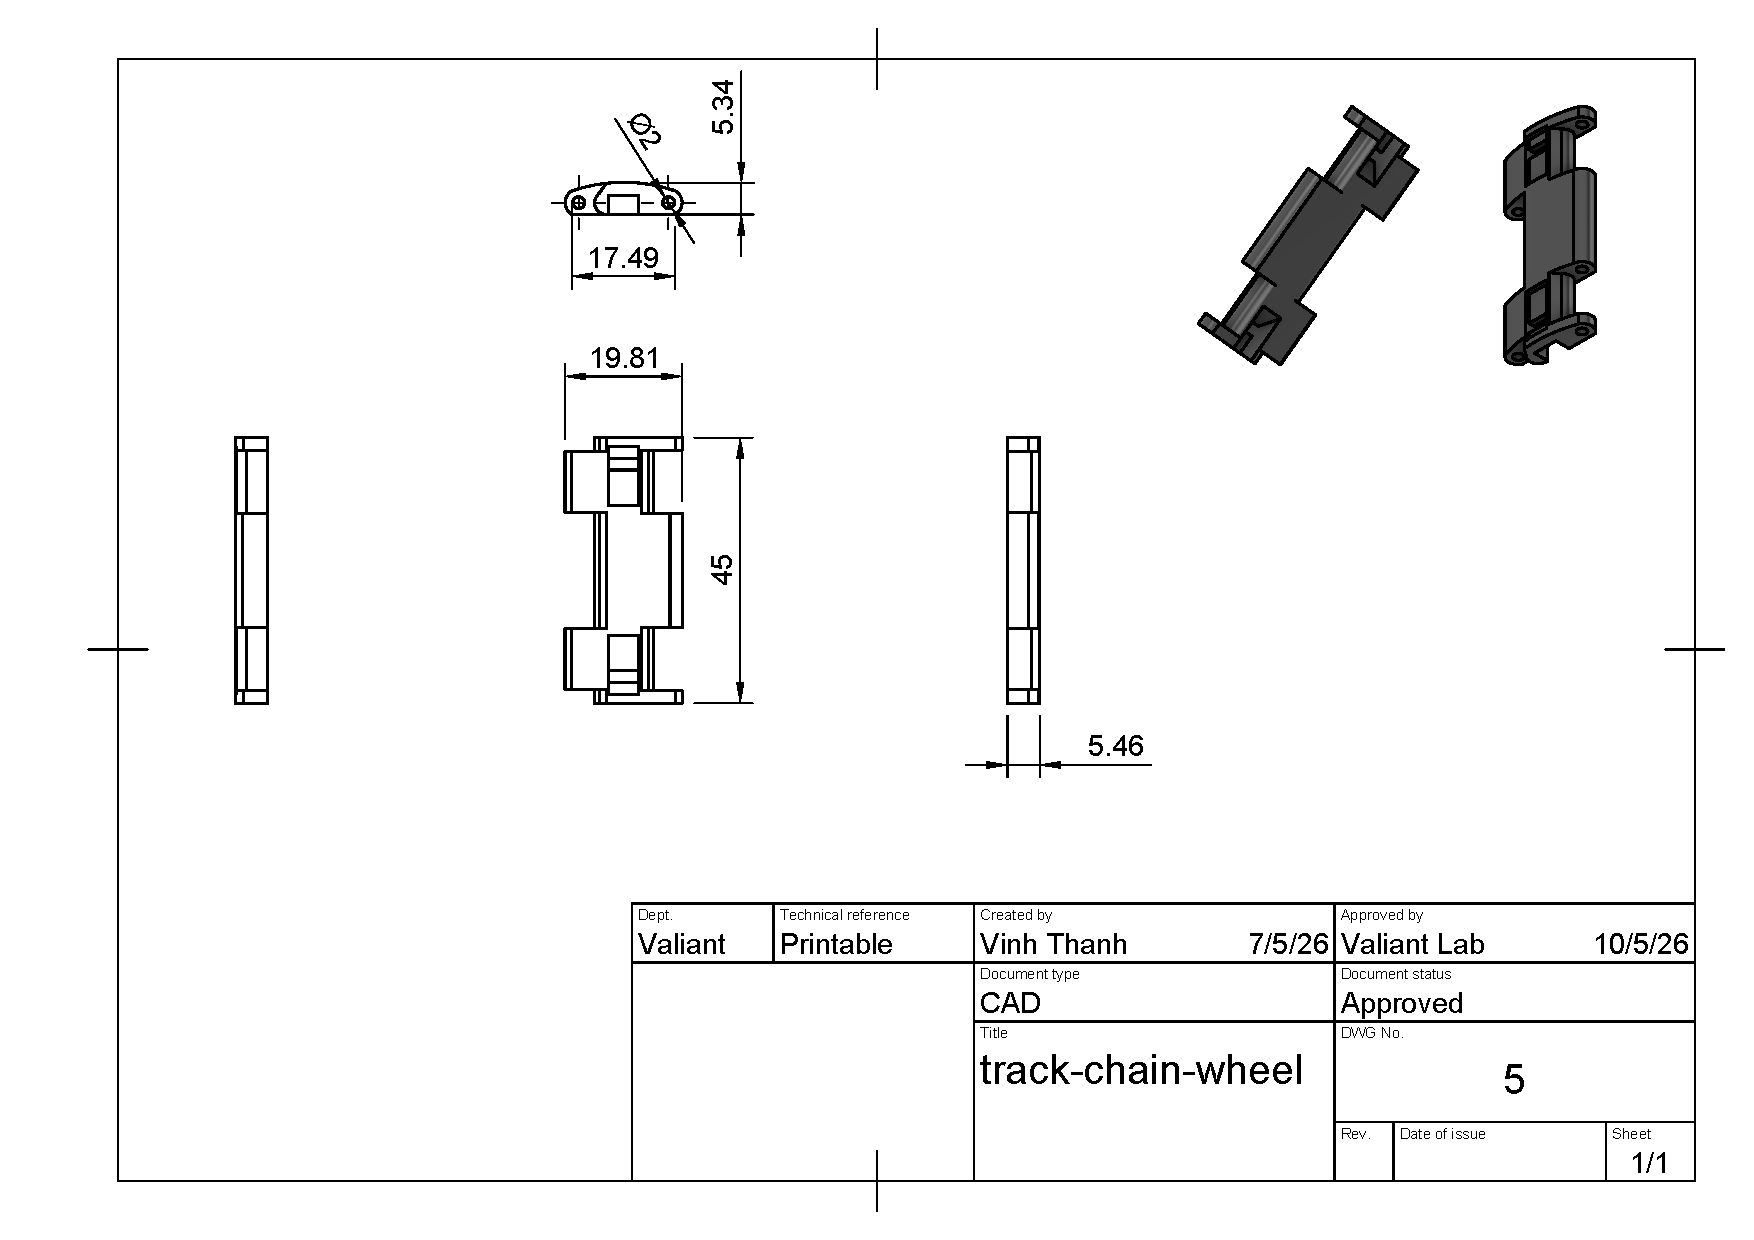
\includegraphics[width=0.75\linewidth]{images/blueprint/track_chain.pdf}
    \caption{Front axis for front wheels for M5 bolts}
    \label{fig:track_chain_blueprint}
\end{figure}\vspace{1em}
\par
MAVEN-01 uses an assembled chain design. In the first design, it used a rubber chain, 
but the wobbling axles caused the rubber track to become unstable, which could lead to 
derailment because there were no stable anchor points for the chain to mount onto both the 
front wheels and the drive wheels, which solved by this second design.

